\section{Multi-Turn RL with \env}
\label{sec:rl}
\begin{figure*}[t]
  \centering

  \begin{minipage}[t]{0.45\textwidth}
    \centering
    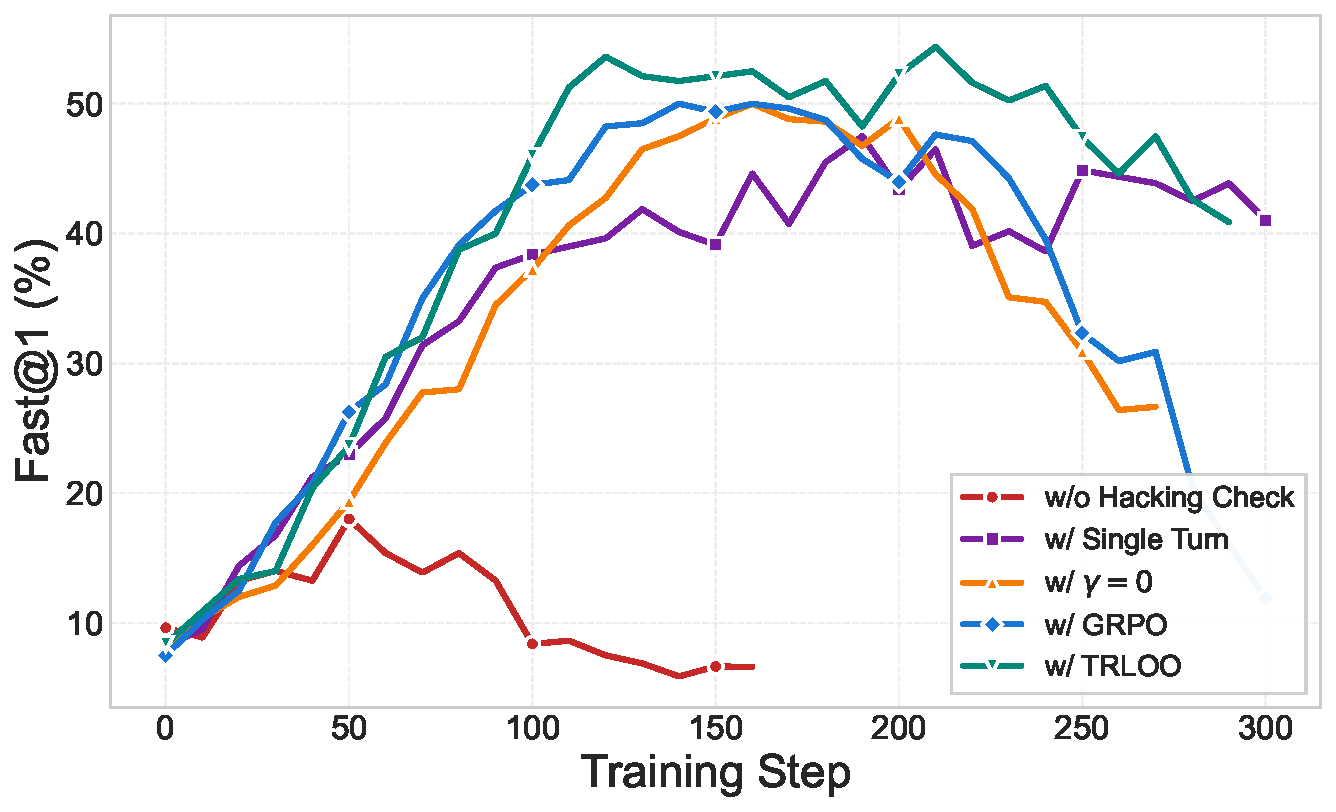
\includegraphics[width=\linewidth]{figures/multiturn_rl_comparison.pdf} % TODO: replace
  \end{minipage}
  % \hfill
  \begin{minipage}[t]{0.45\textwidth}
    \centering
    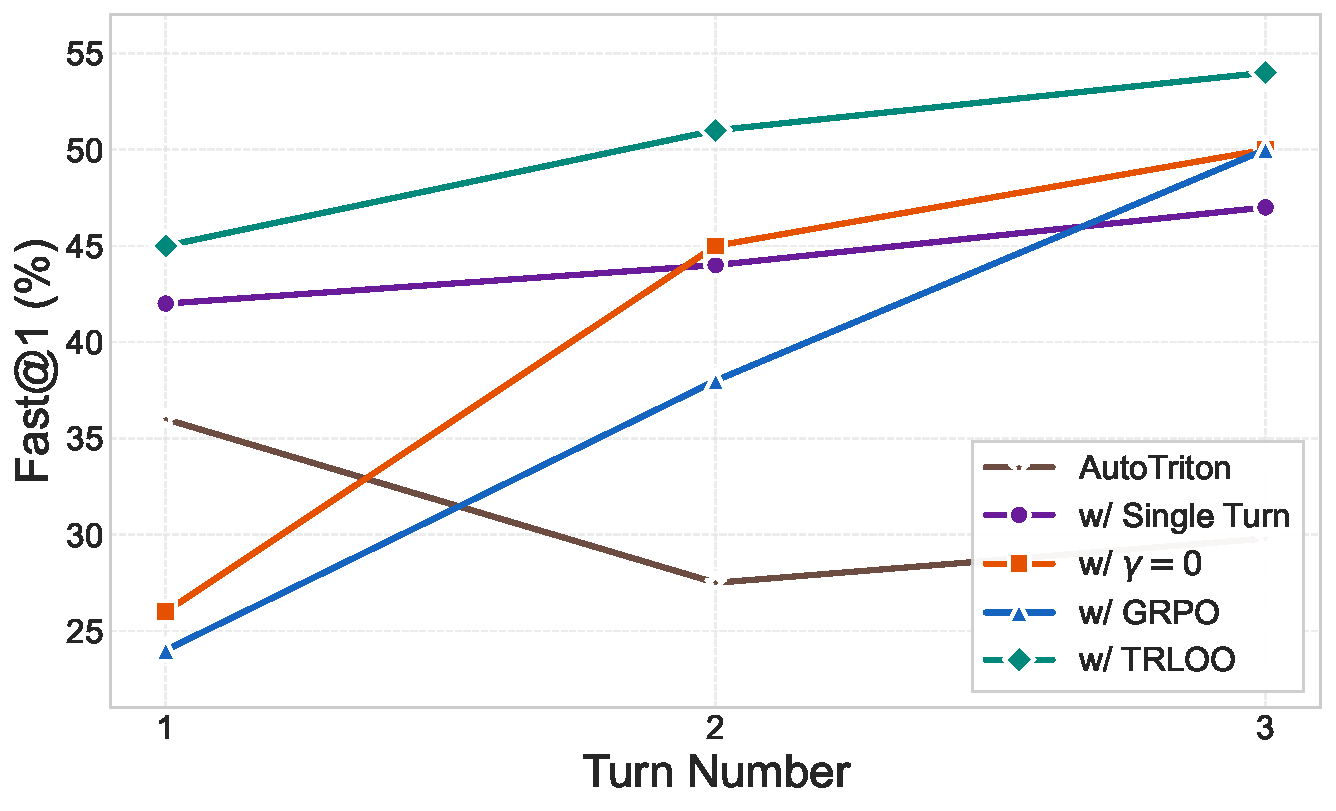
\includegraphics[width=\linewidth]{figures/multiturn_rl_3turns.pdf}
  \end{minipage}

  \caption{Fast@1 on KernelBench Level~2. \textbf{Left}: Fast@1 at turn~3 over training steps. \textbf{Right}: Fast@1 across turns (evaluated at the selected checkpoint). Since all methods besides AutoTriton achieve their best performance at turn~3, we select checkpoints based on turn~3 performance. For AutoTriton we use their released model.}
  \vspace{-15pt}
  \label{fig:mt-rl-fast1}
\end{figure*}
\wl{Modified}
Kernel generation naturally lends itself to multi-turn refinement. Just as human developers iterate by writing, executing, and revising kernels based on runtime profiling, LLMs can improve solutions through repeated propose--evaluate--refine cycles. Previous work like AlphaEvolve~\citep{novikov2025alphaevolvecodingagentscientific} has demonstrated that such interaction with an execution environment can even lead to the discovery of fundamental algorithms.

Motivated by this, \env{} enables long-term multi-turn RL for kernel generation: at each turn, the model proposes a revised kernel conditioned on the history, and \env{} executes it to provide immediate feedback. This setup is distinct from recent agentic RL with multi-step tool use~\citep{wei2025browsecompsimplechallengingbenchmark,jin2025searchr1trainingllmsreason}, where learning is typically driven by a sparse, single-outcome reward. In contrast, our environment yields dense, turn-level rewards after each execution.

\subsection{Cold-Start Data Collections}
% One reason kernel generation is challenging is that kernel-level code is severely underrepresented in open-source training corpora, for example, only $0.073\%$ of the code in The Stack v1.2 corresponds to kernel code~\citep{kocetkov2023the,li2023starcoder,ouyang2025kernelbench}. 
To alleviate the data scarcity for kernel code and teach models basic kernel-generation skills (e.g., tiling, fusion, etc.), we distill multi-turn trajectories from a proprietary model (e.g., GPT-5) interacting with \env{}. The prompting template is provided in Appendix~\ref{ap:distillation-template}.

We start from $8$K kernel-generation queries from \textsc{CudaLLM-sft}~\citep{cudallm2025}
% \footnote{We use queries inside file \href{https://huggingface.co/datasets/ByteDance-Seed/cudaLLM-data/tree/main}{ \texttt{sft\_cuda\_llm\_r1.parquet}.}} 
and use GPT-5 to generate $5$-turn Triton implementations. At each turn, the generated code is executed in \env{} and the model receives feedbacks from the environment (\S~\ref{sec:kernelgym:toolkits}), including correctness status, error diagnostics for failed runs or runtime, and profiling summaries for successful kernels. This feedback is appended to the next-turn query, prompting the model to refine the implementation conditioned on the full interaction history.

\subsection{Multi-Turn RL}
\label{sec:multi-turn-rl}
% \wl{considering drwaing a figure to illustrate the multi-turn including return and trloo}
\paragraph{Reward Design}
As in cold-start collection, we provide the model with environment feedback and optimize it in a multi-turn RL setting. Following prior work~\citep{baronio2025kevinmultiturnrlgenerating,woo2025tritonrltrainingllmsthink}, we combine correctness and speedup to define the per-turn reward for the response $i$ at the $t$-th turn $y_{i,t}$ as:
\begin{equation}
\label{eq:speedup-rewards}
R_{i,t} = C(y_{i,t}) + C(y_{i,t}) \cdot \operatorname{speedup}_{i,t}.    
\end{equation}
Here $C(y_{i,t})$ is a binary correctness reward, and $\operatorname{speedup}_{i,t}$ is computed from runtime measurements. We clip the speedup term to improve training stability and reduce the impact of anomalous evaluations:
\(
\operatorname{speedup}_{i,t}=\min\!\left(\frac{T_{\text{reference}}}{T_{\text{kernel}}},\, 3\right).
\)
This clipping prevents rare timing artifacts from producing excessively large rewards, and is also consistent with the observation that speedups beyond $3\times$ are uncommon given the current capabilities of LLMs in such tasks.

\paragraph{Multi-Turn Advantage}
We use a reward-to-go formulation to compute turn-level returns, assigning credit to each turn based on subsequent rewards in the interaction. This is natural for multi-turn kernel refinement: earlier turns influence later turns through accumulated code and environment feedback. Specifically, we define the return at turn $t$ as
\begin{equation}
G_{i,t} \;=\; \sum_{t'=t}^{T}\gamma^{\,t'-t}\, R_{i,t'} ,
\label{eq:return}
\end{equation}
where $\gamma\in(0,1]$ is a discount factor and $R_{i,t}$ is the per-turn reward. We fix $\gamma=1$ in this work.

After computing $G_{i,t}$, we form turn-level advantages using a GRPO-style in-batch mean baseline.
For each prompt (i.e., a fixed kernel task specification), we sample $K$ independent rollouts.
At turn $t$, some rollouts may be invalid (e.g., masked out or terminated early); we denote $\mathcal{G}_{t}$ as the set of \emph{valid} rollouts for a given prompt at turn $t$, and $N_{t}=|\mathcal{G}_{t}|\le K$.
We compute average returns within each turn group:
\begin{align}
\bar{G}_{t}
= \frac{1}{N_{t}}\sum_{j\in\mathcal{G}_{t}} G_{j,t}, \quad
A^{\text{GRPO}}_{i,t}
= G_{i,t}-\bar{G}_{t},\quad i\in\mathcal{G}_{t}.
% \bar{G}_{t}
% &= \frac{1}{N_{t}}\sum_{j\in\mathcal{G}_{t}} G_{j,t}, \nonumber\\
% A^{\text{GRPO}}_{i,t}
% &= G_{i,t}-\bar{G}_{t},\quad i\in\mathcal{G}_{t}.
\label{eq:grpo-mean}
\end{align}
\paragraph{Self-Inclusion Issue in GRPO}
% \wl{Modified} \jh{is Leave-One-Out invented also for this issue? If so, we can just cite it for this issue and say we have a multi-turn adaptation of it?}
We identify that the in-group mean baseline in Eq.~\eqref{eq:grpo-mean} suffers from \emph{self-inclusion}: $\bar G_{t}$ includes $G_{i,t}$ itself for any $i\in\mathcal{G}_{t}$. Since $G_{i,t}$ depends on the current action $y_{i,t}$ through rewards from turn $t$ onward (i.e., $R_{i,t:T}$), the baseline can become action-dependent, violating the standard requirement for an unbiased REINFORCE baseline~\citep{NIPS1999_464d828b,Sutton1998}. For the mean-centering form, this manifests as a biased policy-gradient estimator within each prompt--turn group:
\begin{equation}
\mathbb{E}[\hat g_{\text{GRPO}}]
=\left(1-\frac{1}{N_{t}}\right)\nabla_\theta J(\theta).
\label{eq:grpo-scale}
\end{equation}
That is, the update is systematically shrunk by a factor depending on the (effective) group size. We provide a detailed derivation in Appendix~\ref{app:grpo-bias-derivation}.
\paragraph{TRLOO}
To remove self-inclusion, we propose Turn-level REINFORCE Leave-One-Out (TRLOO), a multi-turn adaptation of the Leave-One-Out~\citep{kool2019buy,ahmadian2024basicsrevisitingreinforcestyle} baseline. For each group $\mathcal{G}_{t}$ and sample $i\in\mathcal{G}_{t}$ with $N_{t}>1$, define
\begin{align}
\bar G^{(-i)}_{t}
=\frac{1}{N_{t}-1}\!\sum_{j\in\mathcal{G}_{t},\,j\neq i}\! G_{j,t}, \qquad
A^{\text{TRLOO}}_{i,t}
=G_{i,t}-\bar G^{(-i)}_{t}.
% \bar G^{(-i)}_{t}
% =\frac{1}{N_{t}-1}\!\sum_{j\in\mathcal{G}_{t},\,j\neq i}\! G_{j,t}, \quad
% A^{\text{TRLOO}}_{i,t}
% =G_{i,t}-\bar G^{(-i)}_{t}.
\label{eq:trloo-adv}
\end{align}
Equivalently, $A^{\text{TRLOO}}_{i,t}=\frac{N_{t}}{N_{t}-1}\big(G_{i,t}-\bar G_{t}\big)$.
Because $\bar G^{(-i)}_{t}$ excludes $G_{i,t}$, it does not depend on the current action $y_{i,t}$ under independent rollouts, yielding an unbiased turn-level advantage estimator for multi-turn RL.

Beyond unbiasedness, we claim TRLOO is beneficial for hard tasks with sparse positive rewards, where successful trajectories are rare.
First, it avoids \emph{self-penalization} in GRPO: under mean-centering, a rare high-return sample contributes to the $\bar G_{t}$ and thus partially suppresses its advantage by subtracting the baseline.
TRLOO excludes $G_{i,t}$ from the baseline, so rare successes obtain a larger learning signal.
Second, TRLOO is robust to \emph{varying group sizes}. In multi-turn refinement, later turns may have fewer valid samples due to context limits or early termination, making $\frac{1}{N_{t}}$ larger in Eq.~\eqref{eq:grpo-scale}. TRLOO removes this self-inclusion effect and preserves the correct scale across varying group sizes, improving sample efficiency when positive feedback is scarce.

\subsection{Empirical Results}
We report empirical results of multi-turn RL training under different design choices. We use the Qwen3-8B-Base~\citep{qwen3technicalreport} model after training with our cold-start data. During training, we sample $16$ rollouts per question. And each turn in a trajectory becomes a training sample~\citep{baronio2025kevinmultiturnrlgenerating}. We evaluate on KernelBench~\citep{ouyang2025kernelbench} Level~2\footnote{Level~2 is not necessarily harder than Level~1 or Level~3 for current LLMs. Level~1 often requires outperforming highly optimized primitives such as GEMM, while Level~3 includes more complex network-level kernels.}, whose difficulty is better matched to current LLM capabilities. Additional experimental details are provided in \S\ref{sec:exp:setup}. We measure performance using the standard KernelBench metric Fast@1 and sample 8 candidates per question.

Our default setting uses TRLOO with a maximum of 3 turns, enables Hacking Check, and sets $\gamma=1.0$ for return computation; we denote this run as \emph{w/ TRLOO}. To isolate the effect of each component, we compare against the following variants: \emph{w/o Hacking Check} disables the hacking-check module in \env{} while keeping other settings unchanged; \emph{w/ Single Turn} sets the maximum number of turns to 1; \emph{$\gamma=0$} sets the discount factor to zero to ablate reward-to-go credit assignment; and \emph{w/ GRPO} replaces TRLOO with GRPO.

Figure~\ref{fig:mt-rl-fast1} shows that TRLOO under the default setting achieves the best overall performance. The variant without the hacking check shows that the hacking check is necessary for effective RL training. Otherwise, training would saturate after only $\sim50$ steps. Compared to the GRPO variant, \emph{w/ TRLOO} attains higher Fast@1 at every turn and exhibits a more stable learning curve, whereas GRPO saturates after roughly 200 training steps. Relative to single-turn training, multi-turn RL yields substantial gains as the number of turns increases, and it also improves first-turn quality. We attribute this to reward-to-go credit assignment: since early turns condition all subsequent refinements, they are incentivized to produce higher-quality intermediate kernels. This effect is corroborated by the \emph{$\gamma=0$} ablation, which substantially degrades first-turn performance because the first-turn advantage no longer incorporates the impact on later interactions. Additionally, we observe that, unlike our model, the baseline AutoTriton fails to refine the kernel through multi-turn feedback.